% Introduction to SISO Fixed Wireless System Evaluation
\section{Fixed Outdoor SISO System Evaluation}
\label{sec_siso_tvws}

	In this section, we present the planning, design, and evaluation of the first permanent residential \ac{TVWS} communication link inspired by the same frequency-translation radio architecture.
	Utilizing only \ac{SISO} transmission mode with a single antenna and radio, this limited architecture nevertheless provides a reference point for understanding the deployment challenges of TVWS as well as valuable insight regarding the real-world range and performance of TVWS systems.
	At the time of its development and installation in 2011, the installation of a frequency translation-based \ac{TVWS} network represented the first residential TVWS installation in the United States.

%===============================================
\subsection{Frequency Translation Platform for SISO TVWS Connectivity}
\label{sec_freq_xlator_platform}

% ALU Frequency Translator Hardware
\begin{figure}[ht]
\centering
  	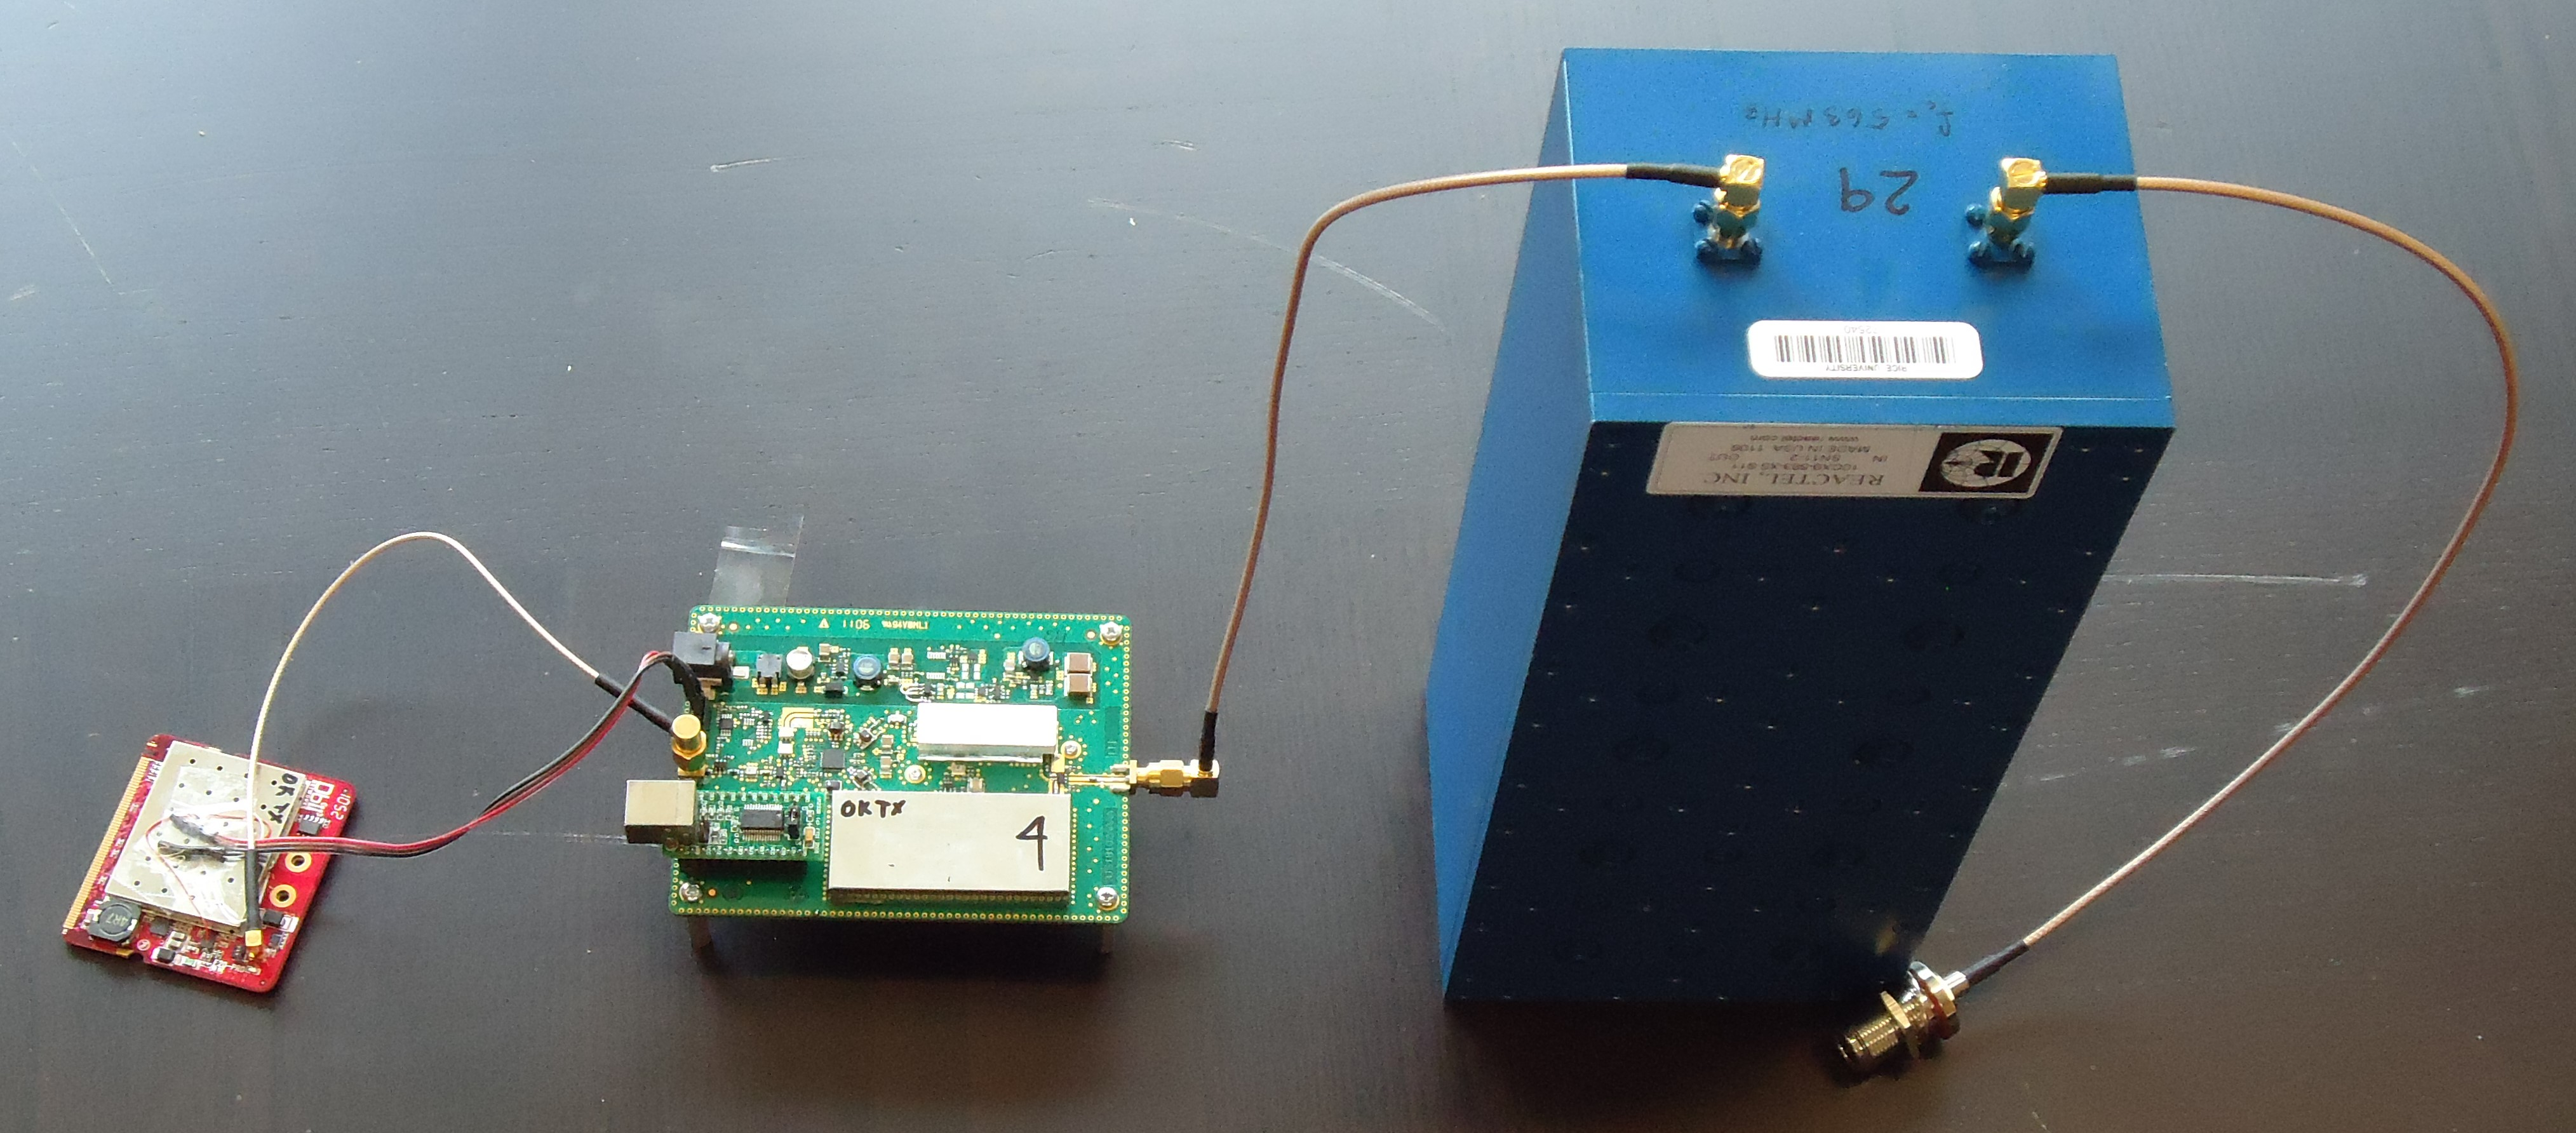
\includegraphics[width=1\linewidth]{figs/wardrive/TFA_translator_chain}   
   	\caption{TVWS frequency translation of 802.11g device.
	\label{fig_freq_translator_hw}}
\end{figure}

	Figure~\ref{fig_freq_translator_hw} shows the main components of the frequency-translator device that we designed.
	From left to right: a 802.11g mini-PCI 2.4~GHz transceiver (red), USB-controlled frequency translator and amplifier from Alcatel-Lucent (green), band-pass resonant cavity filter (blue) providing a 6~MHz passband centered at 563~MHz (UHF channel 29) with approximately 45~dB dropoff into adjacent channels.

%============
\subsubsection{TVWS Spectral Mask}

	The regulatory framework in the United State requires that a \ac{TVWS} transmitter maintain a very sharp spectral mask for radio emissions in order to protect the operation of incumbent broadcast television receivers.
	Figure~\ref{fig_spectral_mask} compares the spectral mask of a \ac{TVWS} transmitter in a single 6~MHz channel (green in-band, red out-of-band) with the mask of an 802.11g 5~MHz transmission.
	The spectral mask of a 20~MHz 802.11g transmitter is also shown in the upper-right section of Figure~\ref{fig_spectral_mask} for comparison.
	In this context, the reference signal strength unit, dBr, can be read as dBc, or signal strength in decibels relative to the desired carrier.

	% FCC Spectral Mask
\begin{figure}[h!]
\centering
  	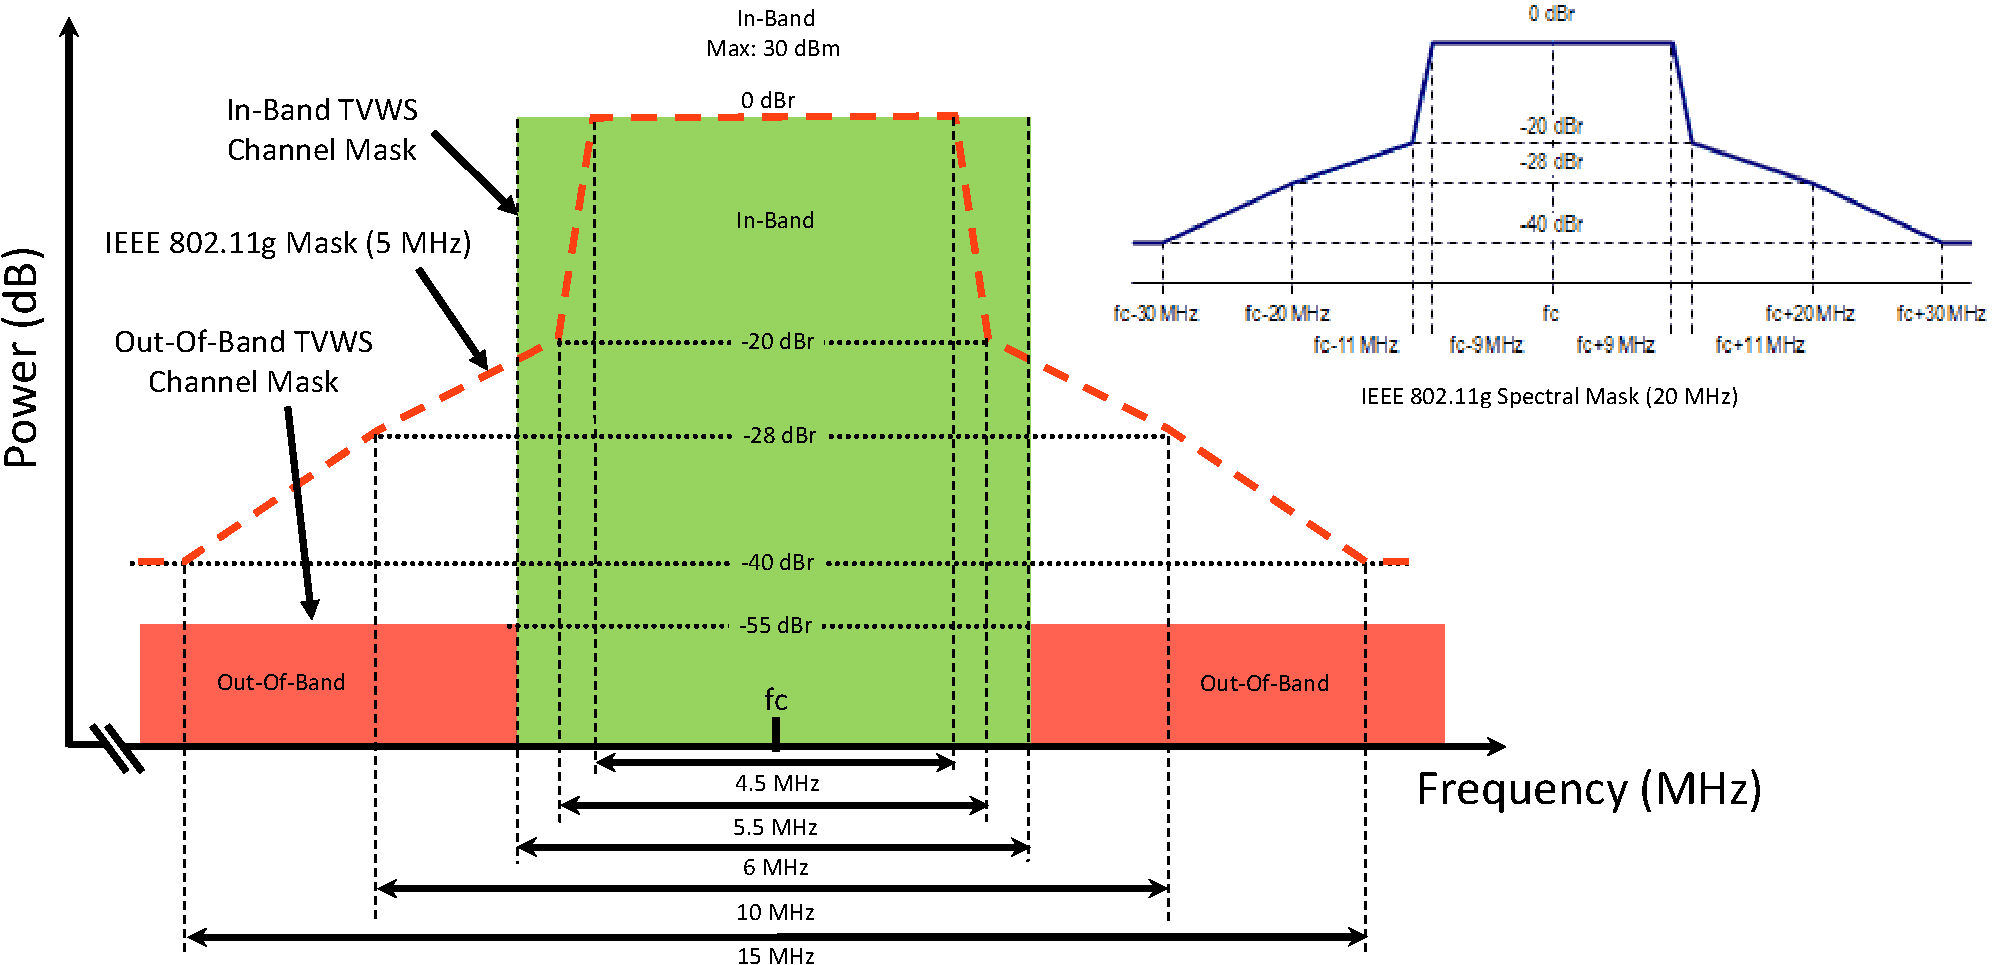
\includegraphics[width=1\linewidth]{figs/wardrive/fcc_spectral_mask}   
   	\caption{Comparison of FCC TVWS spectral mask and 5 MHz 802.11g mask.
	\label{fig_spectral_mask}}
\end{figure}

	Regulations specify that out-of-band power of a \ac{TVWS} device in any 100~kHz slice of spectrum must be less than 72.8~dB below the maximum average in-band power within a 6~MHz channel.
	Assuming a flat power-spectral density, this translates to a -55~dBc out-of-band rejection as shown in Figure~\ref{fig_spectral_mask}.\footnote{802.11 \ac{OFDM} waveforms have a flat power-spectral density, whereas legacy 802.11 \ac{DSSS} waveforms do not.}
	
	This means that any off-the-shelf 802.11-based transmitter will not be able to meet the stringent transmission specifications for a \ac{TVWS} device, requiring the cavity bandpass filter shown in Figure~\ref{fig_freq_translator_hw}.
	
	In addition to controlling the transmit waveform spectral mask, the same high-performance channel bandpass filter is required at the \ac{TVWS} receiver in order to avoid saturating the receiver's \ac{LNA} with high-power out-of-band signals.
		The problem is particularly important with \ac{TVWS} systems where a low-power 40~mW \ac{TVWS} device may be within 12~MHz of a 2~kW broadcast TV station. 
	Out-of-band interference from high-power broadcast transmitters severely decreases the sensitivity and achievable \ac{SINR} of \ac{TVWS} receivers; this phenomenon was observed in multiple deployments during our investigations when bandpass filters were not used.

%============
\subsubsection{Modified 802.11g Driver}

% ALU Frequency Translator PLatform
\begin{figure}[t!]
\centering
  	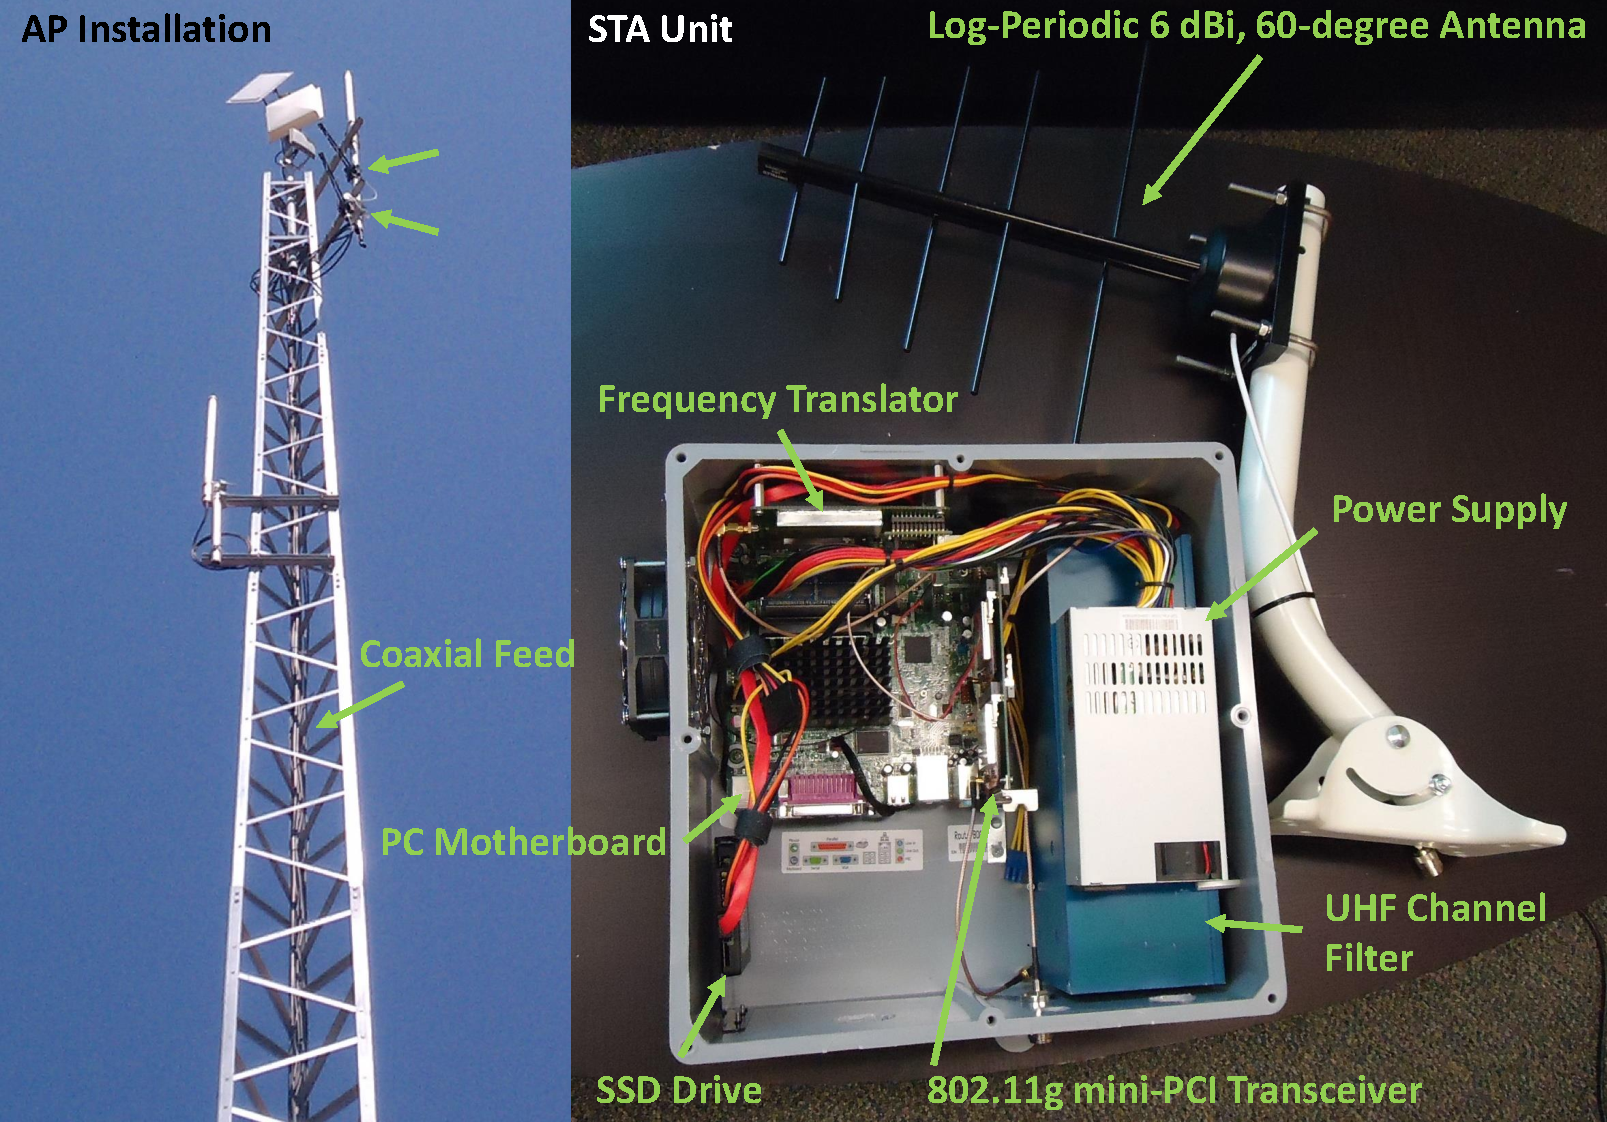
\includegraphics[width=1\linewidth]{figs/wardrive/TFA_translator_platform}   
   	\caption{Integrated TVWS frequency-translation platform and installation.
	\label{fig_freq_translator_system}}
\end{figure}

	Figure~\ref{fig_freq_translator_system} shows the tower installation of a two-sector \ac{TVWS} \ac{AP} with overlapping sector coverage using 6~dBi log-periodic antennas (left), and the completed \ac{TVWS} node with a power supply and embedded x86-based Linux computer platform.
	Each \ac{TVWS} node operates in either \ac{AP} or \ac{STA} mode using a frequency-shifted 802.11b/g Dbii Networks F20-PRO mini-PCI card and a modified open-source ath5k driver that we developed.
	
	The F20-PRO utilized an Atheros AR5414 802.11b/g chipset, which could be controlled with the open-source Linux ath5k driver module.
	While the AR5414 supports multiple channel bandwidths (5/10/20~MHz), at the time the bleeding edge ath5k driver did not.
	We made significant modifications to the ath5k driver in order to first enable these transmission modes and then to control them using the Linux debugfs kernel API \cite{vipin2010analysis}.
	802.11b \ac{DSSS} mode transmissions were disabled in order to meet spectral mask requirements and 802.11 control packets were configured to use 802.11g mode 1: 6~Mbps \ac{OFDM} \ac{BPSK} with coding rate $\frac{1}{2}$.
	In 5~MHz transmission mode on a single 6~MHz \ac{TVWS} channel, this provided a base data rate of 1.5~Mbps.
	Transmission modes up to 802.11g mode 6 (SISO, 16-QAM, 3/4 coding rate) were achievable using this platform in over-the-air \ac{TVWS} channels, with a theoretical maximum data rate of 9~Mbps. Rates up to 7~Mbps were regularly achieved during our trials.
	
	Additional driver modifications were included to extract \ac{PHY} and \ac{MAC}-layer parameters, such as the number of re-transmissions, source and destination node, received signal strength, and estimated channel noise floor.
	These parameters were recorded for each received packet, providing enhanced cross-layer information beyond that reported by wireless Linux drivers at the time.
	
	All \ac{TVWS} frequency-translator nodes used this modified driver and additional command and control scripts to deploy a fixed 802.11 infrastructure network using available \ac{TVWS} channels in Houston.
	The modified driver code is available open-source on GitHub \cite{guerra2013ath5kmod}.
	
\subsubsection{Cognitive Radio Sensing Technique}
	Whereas the Microsoft KNOWS platform \cite{narlanka2007hardware} utilized a separate built-in spectrum analyzer for determining TVWS channel vacancies, we instead chose to rely on shared spectrum database lookup as the enabling cognitive radio technology \cite{flores2013ieee80211af}.

	In order to meet the primary user detection thresholds required of TVWS systems, simple energy detection is not sensitive enough to protect incumbent broadcast television stations within their geographic protection contours \cite{wu2000comparison, gautier2011cyclostationarity, shellhammer2008spectrum}.
	The regulatory protection contour \cite{hessar2015capacity} for a digital broadcaster within the United States is the geographic region defined by the 41~dBu~F(50/90) contour, or the region where 50\% of locations will have a signal strength greater than the given dBu value 90\% of the time.
	A dBu is legacy unit that is a decibel measure of the \ac{RMS} voltage level referenced to 0.775~Vrms.

	Rather than implement more complex feature detection \cite{shellhammer2008spectrum} or experimental cooperative spectrum sensing \cite{mishra2006cooperative}, we instead choose to utilize a centralized national spectrum database for experimental planning and regulatory compliance.
	Since the input to a spectrum database lookup is a geolocation and the database directly estimates primary user protection contours utilizing the same propagation models used to determine those contours, it is a more reliable method for primary user protection than direct spectrum sensing when radio devices have access to that database.

	This choice of synchronization technology reduces the amount of engineering effort in system design while providing reliable protection for primary users.
	As of today, database synchronization remains the only cognitive radio technology in use for TVWS devices.

%===============================================
\subsection{TVWS Channel Availability and Selection}
\label{sec_tvws_chan_availability}

	\ac{TVWS} radios are allowed to determine what available white space radio spectrum is available through one of two methods: 1) location-based lookup in a national radio spectrum database; or 2) sensing the presence of an incumbent television broadcaster with signal strength below -114~dBm over a 100~kHz window.\footnote{A received signal strength above -114~dBm in any 100~kHz window indicates that a channel is ``occupied'' by an incumbent and can not be considered a ``white space.''}
	When planning the installation of a new \ac{TVWS} network in Houston, we chose to test database predictions against radio spectrum sensing to better understand the accuracy of the database as well as potential noise or interference on UHF channels.
	
	% Locations of Spectrum Scan
\begin{figure}[ht]
\centering
  	\includegraphics[width=1\linewidth]{figs/wardrive/houston_scan_locs}   
   	\caption{Scan locations (yellow pins) in the Houston metropolitan area, December 2010.
	\label{fig_houston_scan_locs}}
\end{figure}

	Power spectral density measurements were taken at diverse locations in the Houston metropolitan area using an Agilent e4402b spectrum analyzer with a 100~kHz resolution bandwidth and 100~point \ac{RMS} power average.
	The scan location are marked as yellow pins in Figure~\ref{fig_houston_scan_locs}.
	
	This measurement was repeated with two different antennas: a Fractal UACM-V 150-6000~MHz omnidirectional fractal antenna and a Radio Shack Model ``20-032'' 25-1300~MHz omnidirectional whip antenna, both with approximately 0~dBi gain across their sensitivity range.
	The observed power spectral density at these locations measured between 08:00 and 19:00 on December 15, 2010 is displayed in Figure~\ref{fig_all_spectrum_occupancy}, showing significant under-utilization of radio resources in the Houston area.
	The large empty section between 235-440~MHz is reserved for fixed mobile space communications and radio-navigation applications, with the active sections between 440-470~MHz for fixed mobile, radio-navigation, satellite, and medical radio applications \cite{fcc2018spectrumtable}.
	
	We focus on our UHF band of interest, 470-698~MHz in Figure~\ref{fig_uhf_channel_availability}, where we display the UHF channelization numbers (black numbers 14-51), 6~MHz channelization boundaries (dashed red lines), and the mean and standard deviation of the observed power spectral density across all measurement locations to demonstrate the range of observations.
	
% All Spectrum Scan
\begin{figure}[ht!]
\centering
  	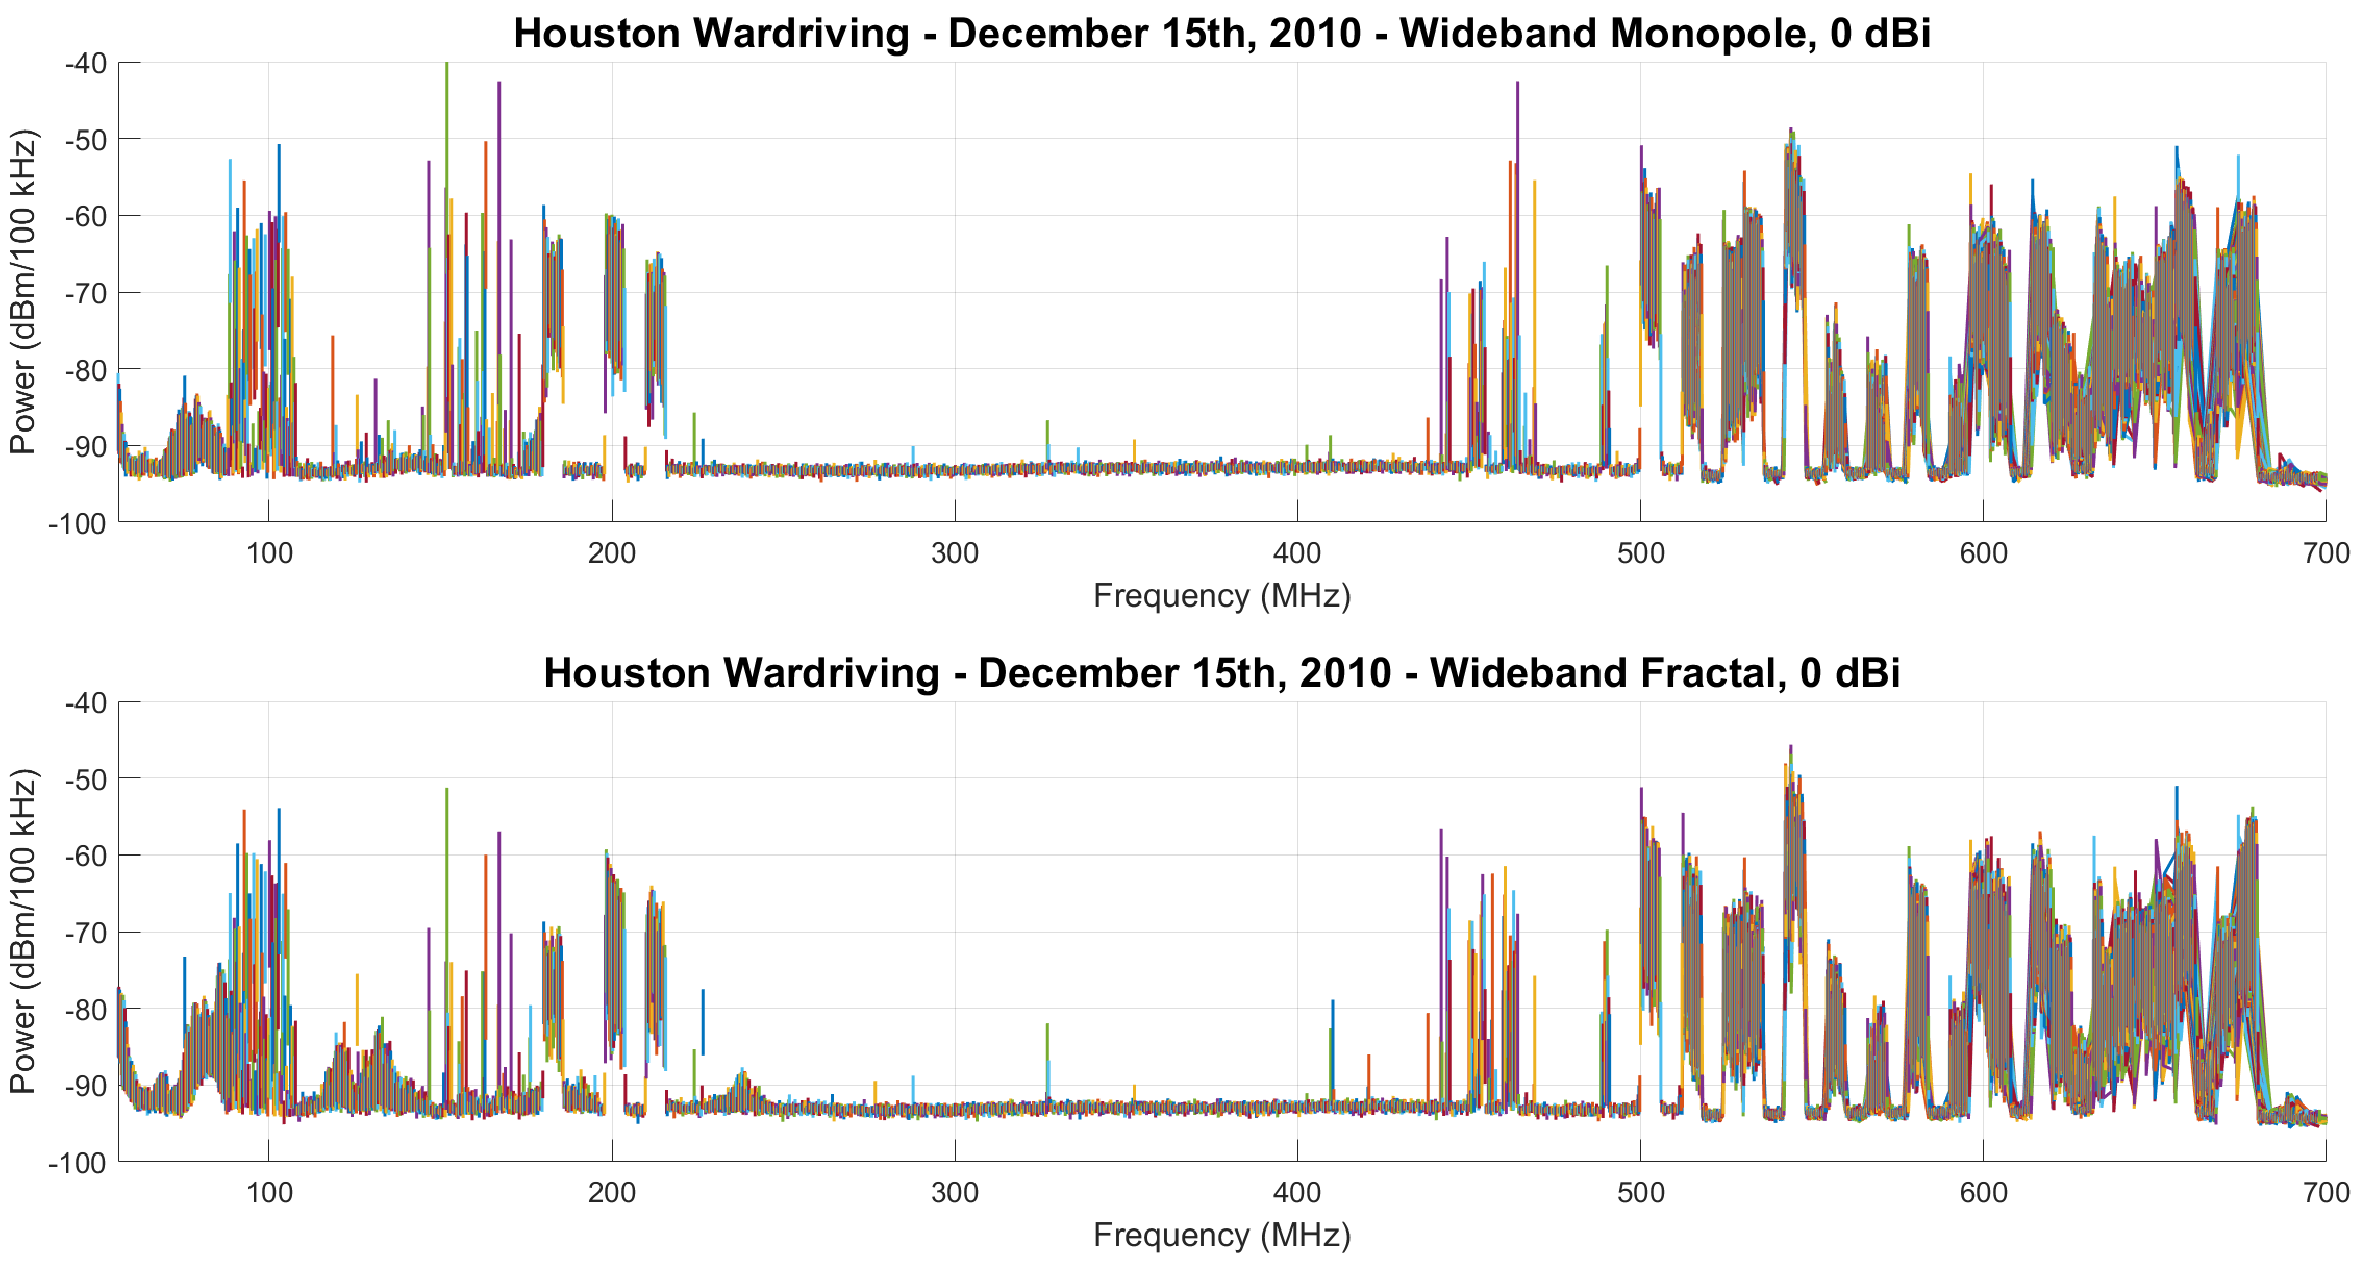
\includegraphics[width=1\linewidth]{figs/wardrive/Houston_Wardriving_12_17_2010_v2}   
   	\caption{Measured VHF/UHF occupancy in the Houston metropolitan area, Dec 2010.
	\label{fig_all_spectrum_occupancy}}
\end{figure}

% UHF Spectrum Channelization
\begin{figure}[ht!]
\centering
  	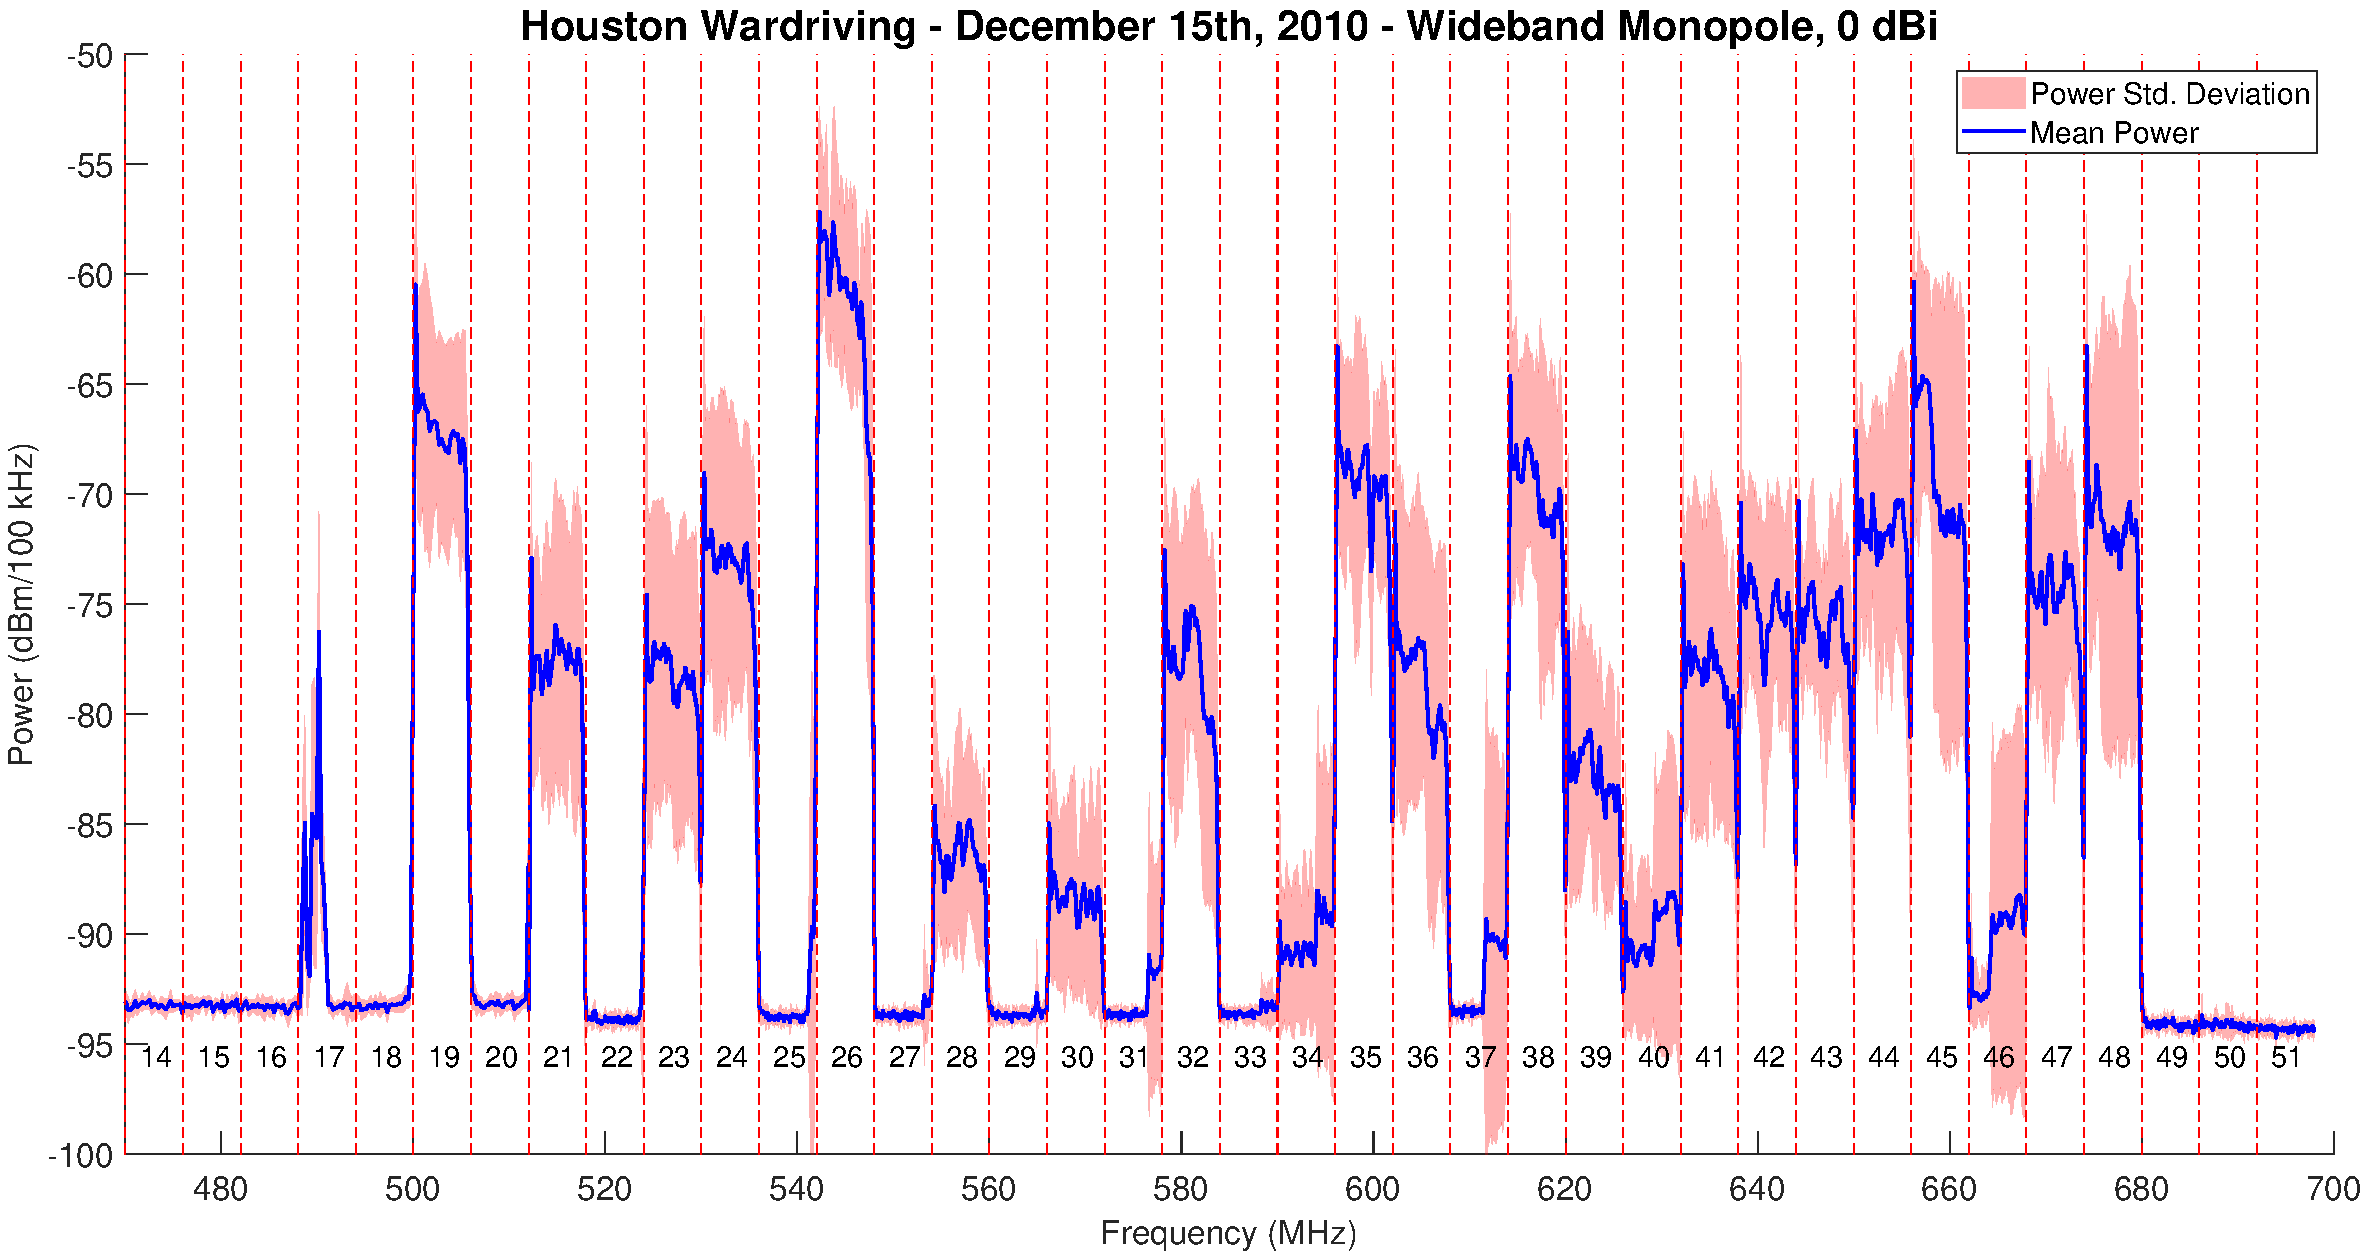
\includegraphics[width=1\linewidth]{figs/wardrive/Houston_UHFOnly_12_17_2010}   
   	\caption{Measurement UHF channel occupancy in Houston metropolitan area, December 2010.
	\label{fig_uhf_channel_availability}}
\end{figure}

	We show that channel occupancy in the Houston area has approximately 9 channels that may be available for secondary \ac{TVWS} reuse below channel 37.\footnote{In March 2016, the FCC performed the first reverse-spectrum auction to re-allocate all radio spectrum above UHF channel 37 for licensed purposes \cite{gomez2015broadcast}, thus removing it from consideration for \ac{TVWS} purposes. Notable exclusions are the 652-663~MHz ``duplex gap,'' which may become available for \ac{TVWS} operation, and channel 37, which is reserved for medical telemetry. These frequent changes to spectrum policy and future uncertainty provides additional motivation for agile, software-defined \ac{TVWS} platforms.}
	Confirmation of channel vacancy was provided by certified spectrum databases from Google, Spectrum Bridge, and Telcordia.
	Vacancy of a primary transmitter combined with the low power of the adjacent-channel primary broadcasters on channels 28 and 30 led us to select channel 29 for deployment of our trial \ac{TVWS} network.
	
%%====================
%\subsubsection{Updates to TVWS Availability} \label{sec_tvws_regulation}
%\rgnote{Discussion regarding regulatory changes since the initial measurements were taken.}

%===============================================
\subsection{TVWS Fixed Wireless SISO Coverage}
\label{sec_tvws_fixed_siso}

	The neighborhood of Pecan Park is primarily residential, consisting of low-income households in the Houston, TX East End region \cite{camp2006developing}.
	Previously, a hybrid wireless 2.4~GHz/5.8~GHz 802.11a/b/g network was established utilizing a two-tier 802.11s mesh topology, blanketing the approximately 20,000 residents with wireless coverage and access throughput up to 6~Mbps \cite{camp2006measurement, camp2008measurement}.\footnote{At the time, the access tier utilized 802.11b \ac{DSSS} technology, with a maximum 11~Mbps \ac{PHY} rate. Higher \ac{PHY} rates would almost certainly be achievable with modern 802.11n/ac/ax technology utilizing the same link budget.}
	In this section, we directly evaluate the performance of an 802.11af-like network overlay in the same neighborhood in order to compare and contrast \ac{TVWS} system performance with other \ac{ISM}-band alternatives.

% ##################
\subsubsection{Expected Model Performance}
\label{sec_hata_model}

	We wish to generate a first approximation of the expected coverage range of a \ac{TVWS} network within the Pecan Park neighborhood in order to plan network deployments.
	While more detailed propagation models such as the Longley-Rice terrain-based model are available, we focus first on the Hata-Davidson curve-fitting model as a more simple model with relatively good accuracy in \ac{TVWS} bands \cite{kasampalis2014comparison}.
		
	We estimate the maximum distance from a 20~meter transmitter to a 3~meter receiver when the transmit power is 30~dBm and the receiver’s minimum sensitivity is -80~dBm as a function of the transmit frequency and display the resulting maximum distance of coverage in Figure~\ref{fig_hata_model}.
	Sensitivity of -80~dBm approximately matches the receive performance of the frequency-translation system presented in Section~\ref{sec_freq_xlator_platform}.
	Free-space propagation curves are also displayed for the previously reported free-space path loss exponent of $\gamma = 3.3$ for the same region \cite{camp2006measurement}, and we highlight the intended center frequency of operation in the Pecan Park installation as the vertical red line at 563~MHz.
		
	Based on the model predictions, we can expect the maximum range under Hata propagation to be approximately 1300~meters and approximately 600~meters utilizing the previously observed path-loss value of $\gamma = 3.3$.
	We shall see in the next section how well these model predict propagation behavior.
		
		
% Hata/Free Space Models
\begin{figure}[ht!]
\centering
  	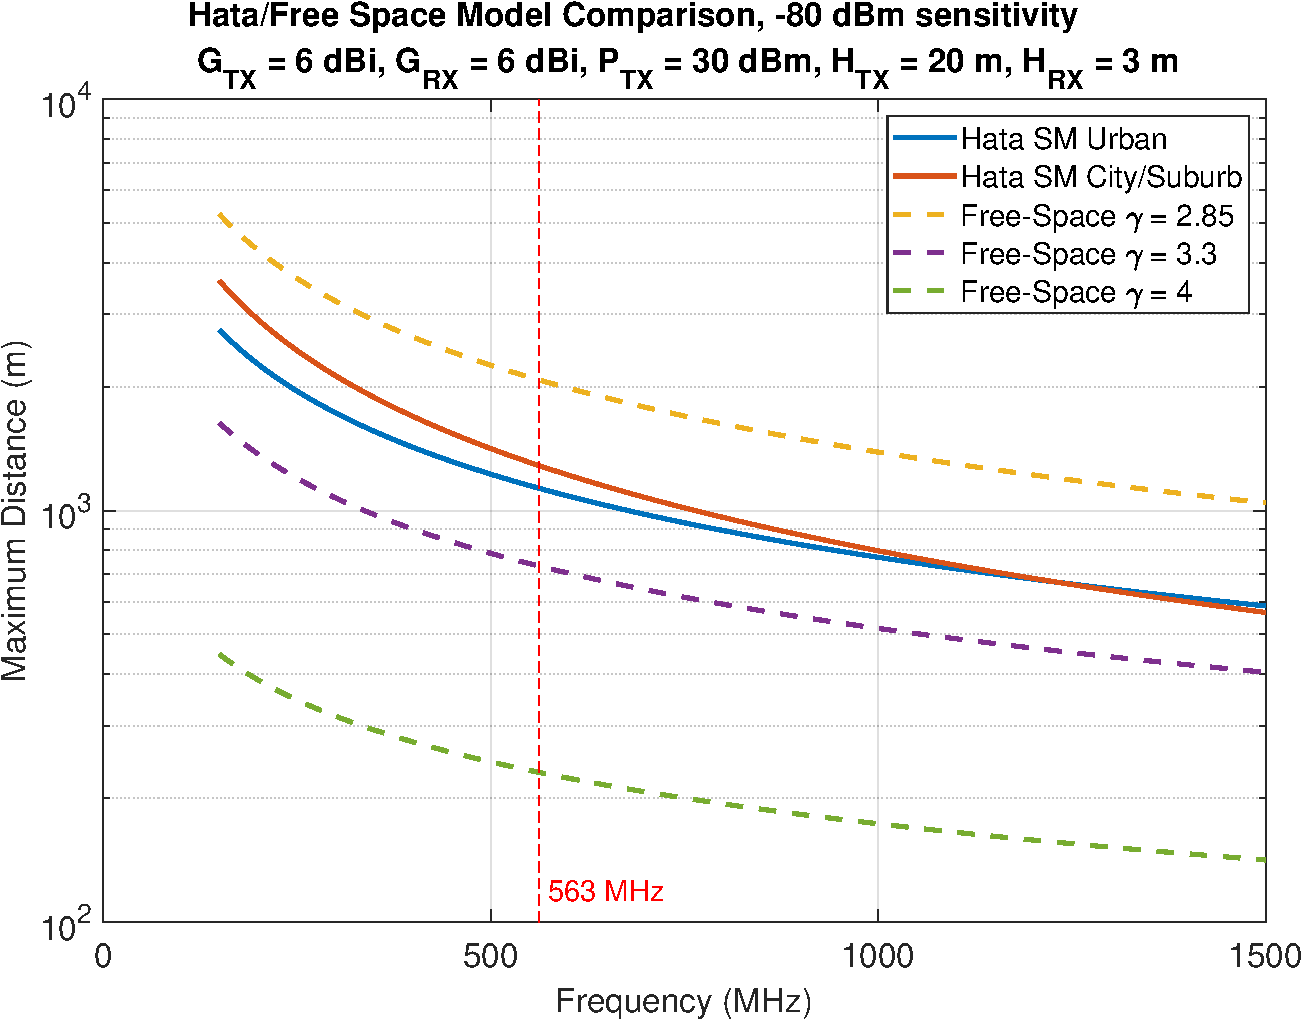
\includegraphics[width=0.8\linewidth]{figs/wardrive/Hata_v_FreeSpace_11_02_2018}   
   	\caption{Expected maximum -80~dBm receive range using Hata and Free-Space models.
	\label{fig_hata_model}}
\end{figure}

% ##################
\subsubsection{Measured Performance}
\label{sec_tfa_wardrive_performance}
	
% TFA Wardrive Coverage Visualization
\begin{figure}[ht]
\centering
  	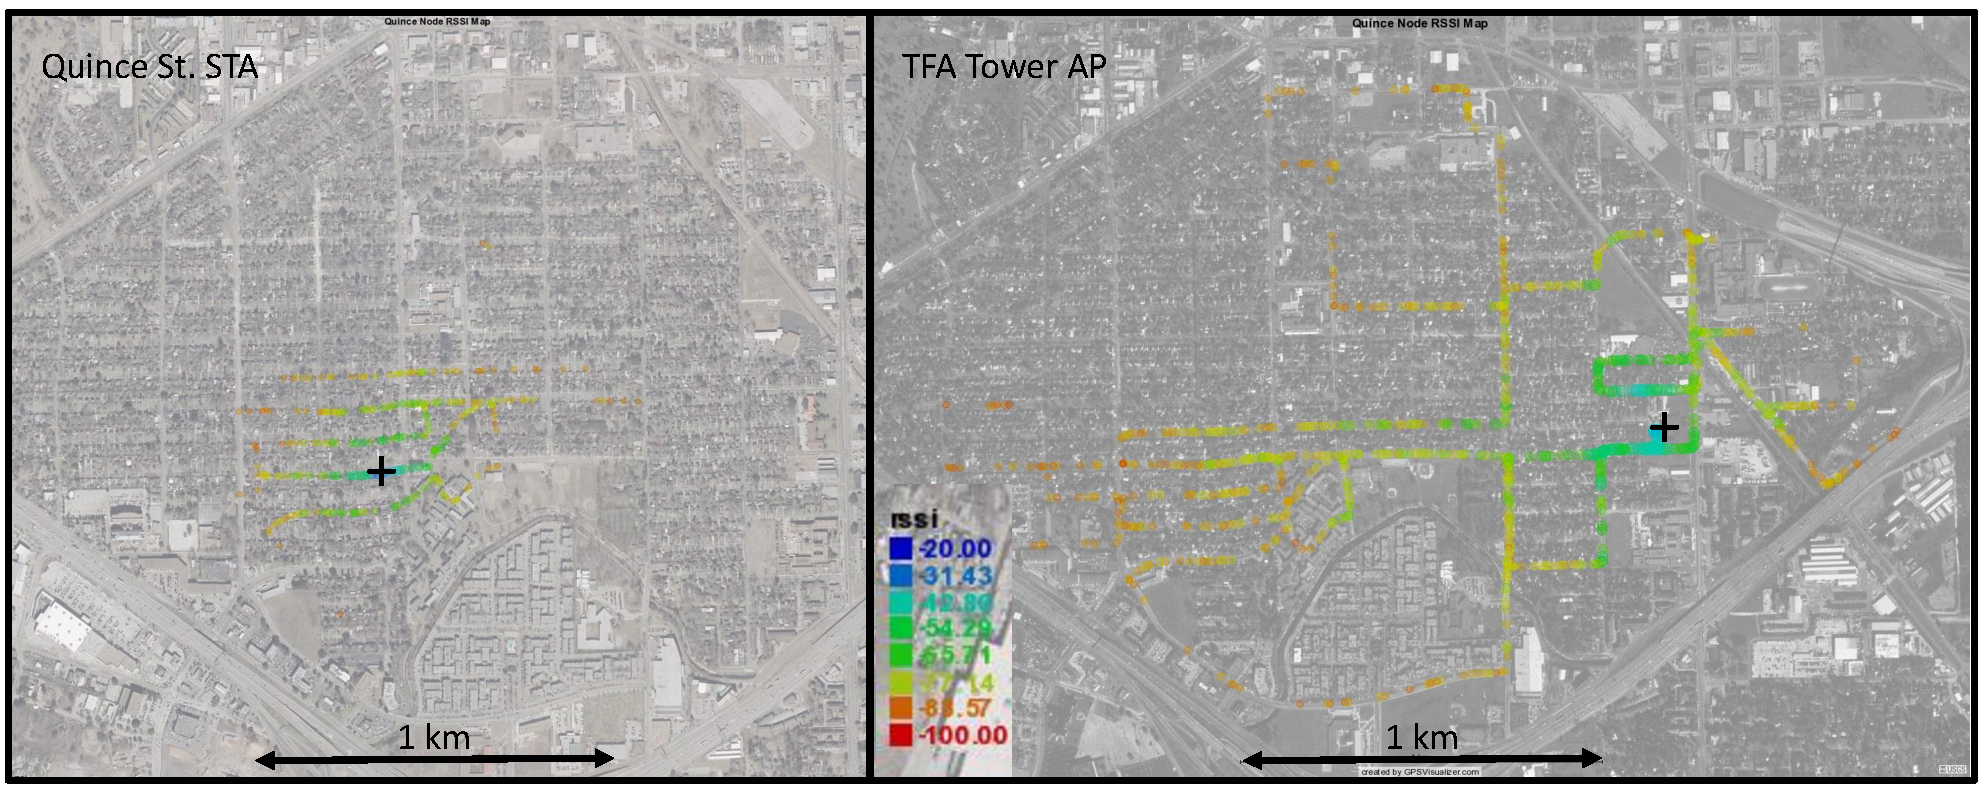
\includegraphics[width=1\linewidth]{figs/wardrive/TFA_wardrive_coverage}   
   	\caption{Measured RSSI coverage map of TFA \ac{SISO} \ac{TVWS} installation, \ac{AP} and \ac{STA}.
	\label{fig_uhf_rssi_map}}
\end{figure}

	In order to test the coverage range and expected achievable rate, we deployed two overlapping \ac{AP} sectors of \ac{TVWS} coverage (black log-periodic antennas in Figure~\ref{fig_freq_translator_system}) utilizing the frequency-translation system introduced in Section~\ref{sec_freq_xlator_platform} on a 20-meter tower.
	In addition, a permanently installed \ac{STA} was similarly configured, except it was installed under-the eaves of a residential home at a height of approximately 3~meters.
	Both \acp{AP} and the \ac{STA} were configured with 6~dBi log-period 400-700~MHz antennas.
	Each node was configured to transmit broadcast beacons once per second at the lowest \ac{PHY} rate.
	An additional listener \ac{STA} node configured in promiscuous mode (to avoid the need to maintain association with the \ac{AP}) was driven at 5~MPH within the expected coverage region utilizing the same 0~dBi whip antenna as in Section~\ref{sec_tvws_chan_availability} mounted on the roof of the car at approximately 1.5~meters height.

	A visual representation of the received signal strength from both the \ac{STA} and \ac{AP} at the mobile car receiver is shown in Figure~\ref{fig_uhf_rssi_map} for all measurement points.

% TFA Wardrive Pathloss and Range Estimation
\begin{figure}[p]
\centering
  	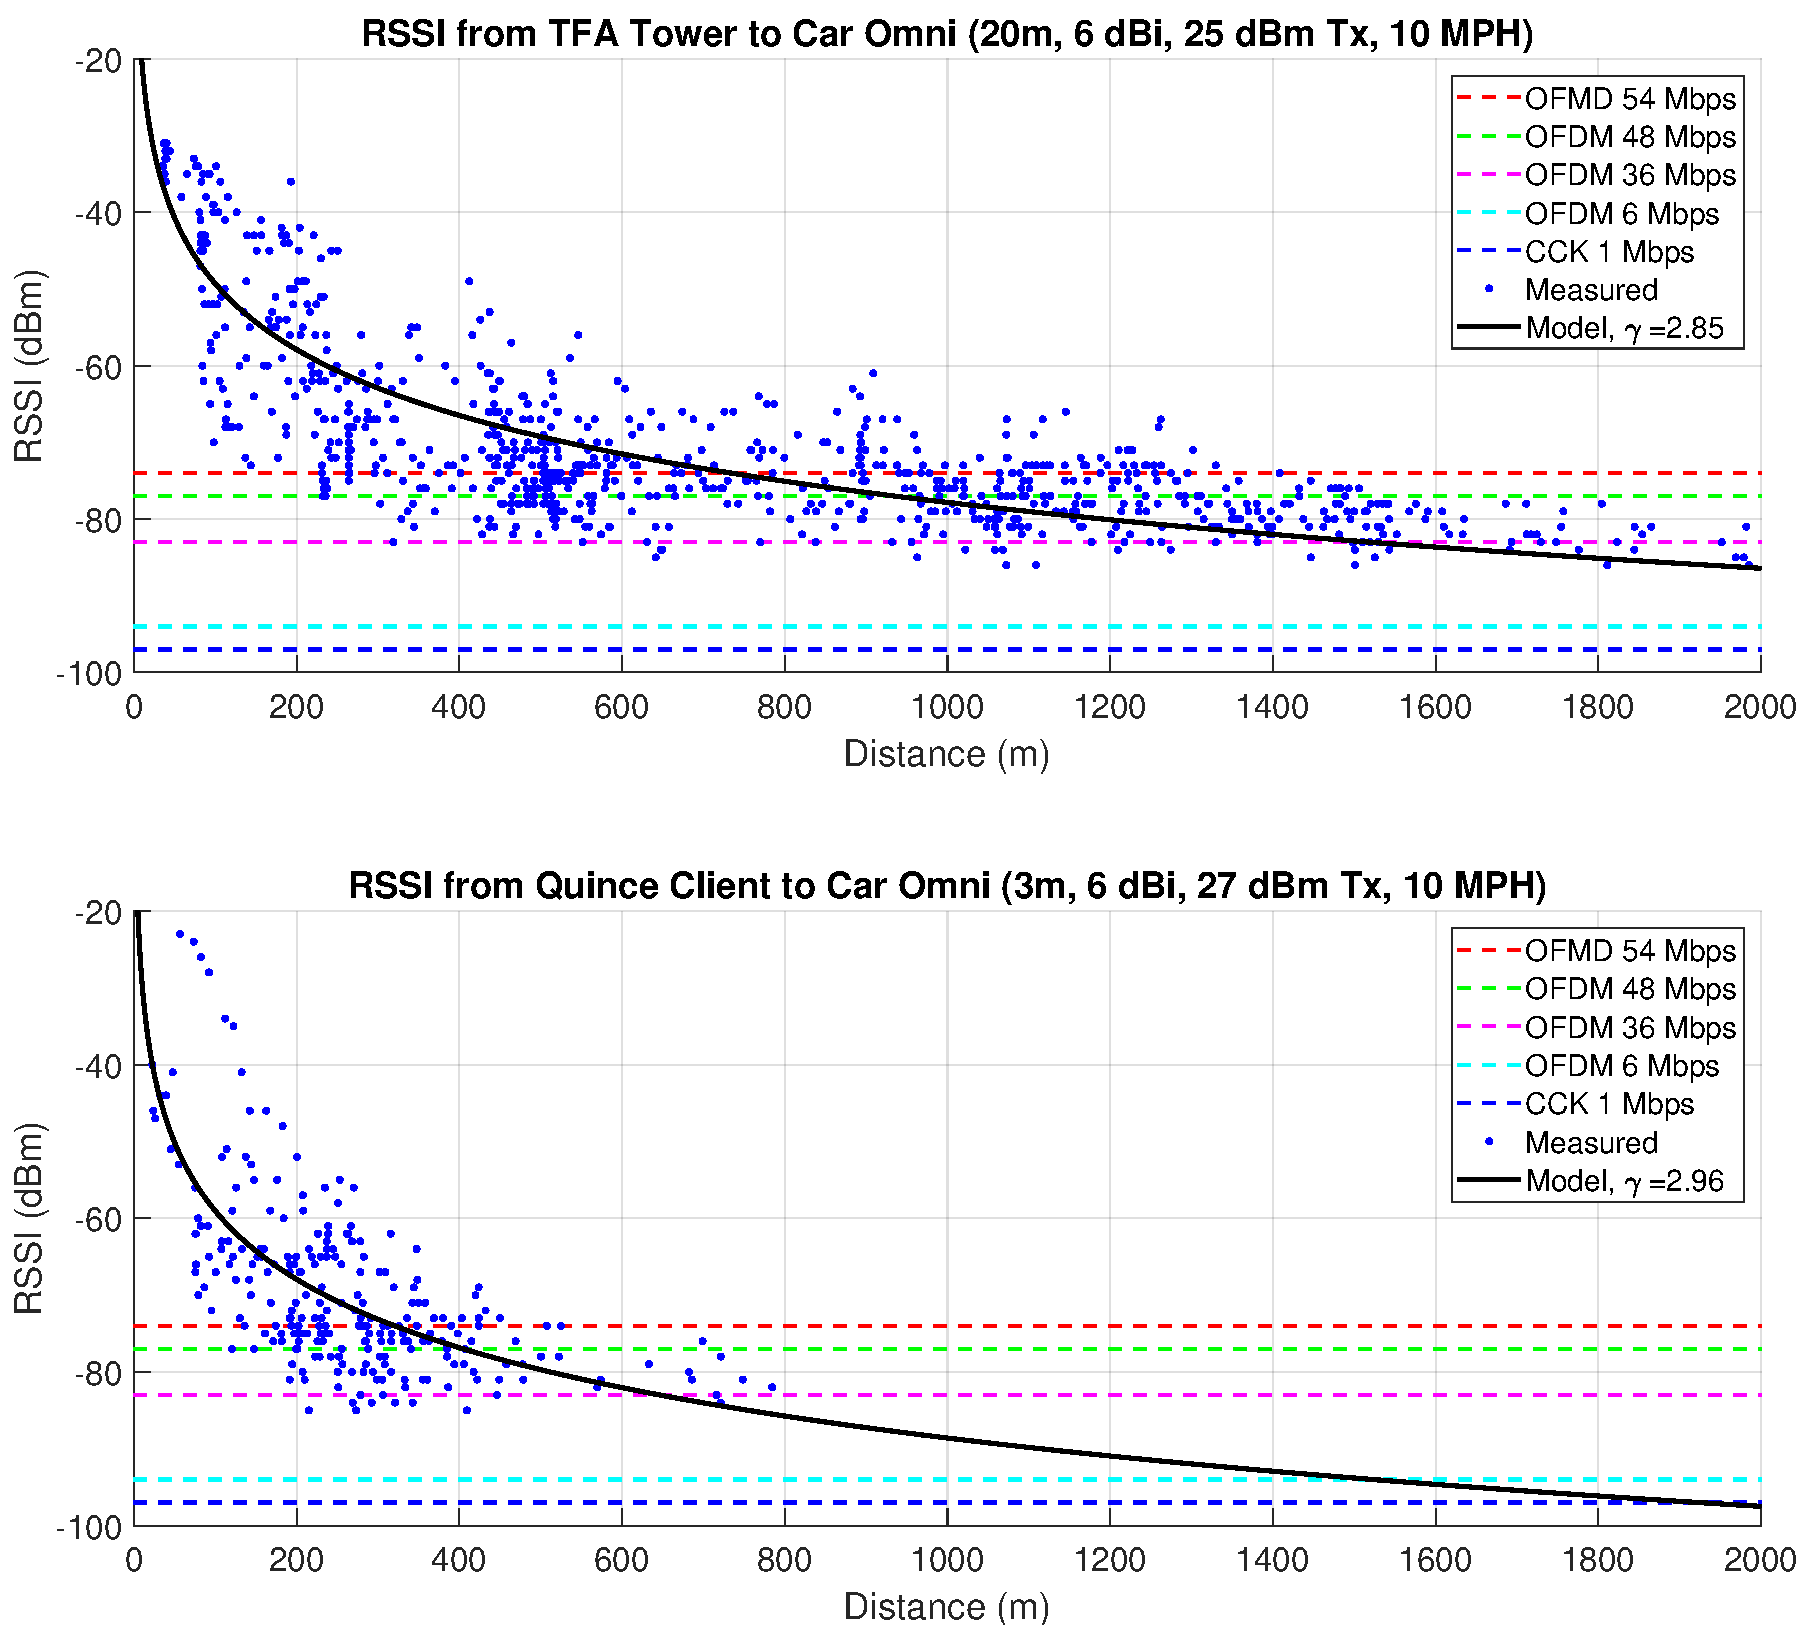
\includegraphics[width=1\linewidth]{figs/wardrive/TFA_Wardrive_Pathloss}   
   	\caption{Free-space pathloss model fitting of TFA \ac{SISO} \ac{TVWS} installation.
	\label{fig_uhf_siso_fspl}}
\end{figure}

	We observe much improved coverage distance utilizing the 563~MHz 802.11af-like system compared to the legacy 2.4~GHz previously installed in the same environment, as expected from the comparison in \cite{flores2013ieee80211af}.
	For example: the mean -80~dBm reception radius was approximately 300~m within the same environment with the previous 2.4~GHz network \cite{camp2006measurement}, whereas we observe a mean -80~dBm reception distance radius of approximately 1.15~km from the \ac{AP} as observed for the \ac{TVWS} network (Figure~\ref{fig_uhf_siso_fspl}, tower modeled curve).
	In terms of network planning impact, coverage of the Pecan Park neighborhood was projected to require 30 2.4~GHz mesh nodes to serve nomadic and residential users \cite{camp2006developing, camp2008measurement} using a two-tier topology; a single-tier network utilizing \ac{SISO} \ac{TVWS} could cover the entire region with \ac{NLoS} coverage using only 2-4 nodes, representing the potential for significant cost savings.
	
	We also plot the sensitivity threshold for various 20~MHz 802.11g \ac{PHY} layer rates in Figure~\ref{fig_uhf_rssi_map}.
	This provides an estimate regarding the 802.11g/af \ac{PHY} layer rates that would be available at various distances from a commercial \ac{TVWS} system should the channel bandwidth be increased from 5~MHz to 20~MHz, or from a single 6~MHz UHF channel to 4 bonded channels with 24~MHz total channel bandwidth.

%===============================================
\subsection{TVWS Long-term Channel Stability}
\label{sec_tfa_stability}

	A common expectation of large-scale \ac{TVWS} is that there may be fluctuations in performance due to a number of potential sources: 1) ionosphere bounce propagation, which should only be apparent below 20~MHz; 2) tropospheric irregularities where diurnal temperature cycles and random weather effects can produce weak dielectric changes in the troposphere, resulting in wave reflections; 3) swaying or movement of the tower and antennas; and even 4) extreme phenomenon such as meteor-burst effects \cite{raab2002hf}.
	These effects could be apparent in the desired signal as well as varying the environmental noise floor.
	Therefore, we configure a longitudinal series of \ac{RSSI} and noise floor measurements using the installed infrastructure in order to test this hypothesis.

% TFA Channel Stability
\begin{figure}[p]
\centering
  	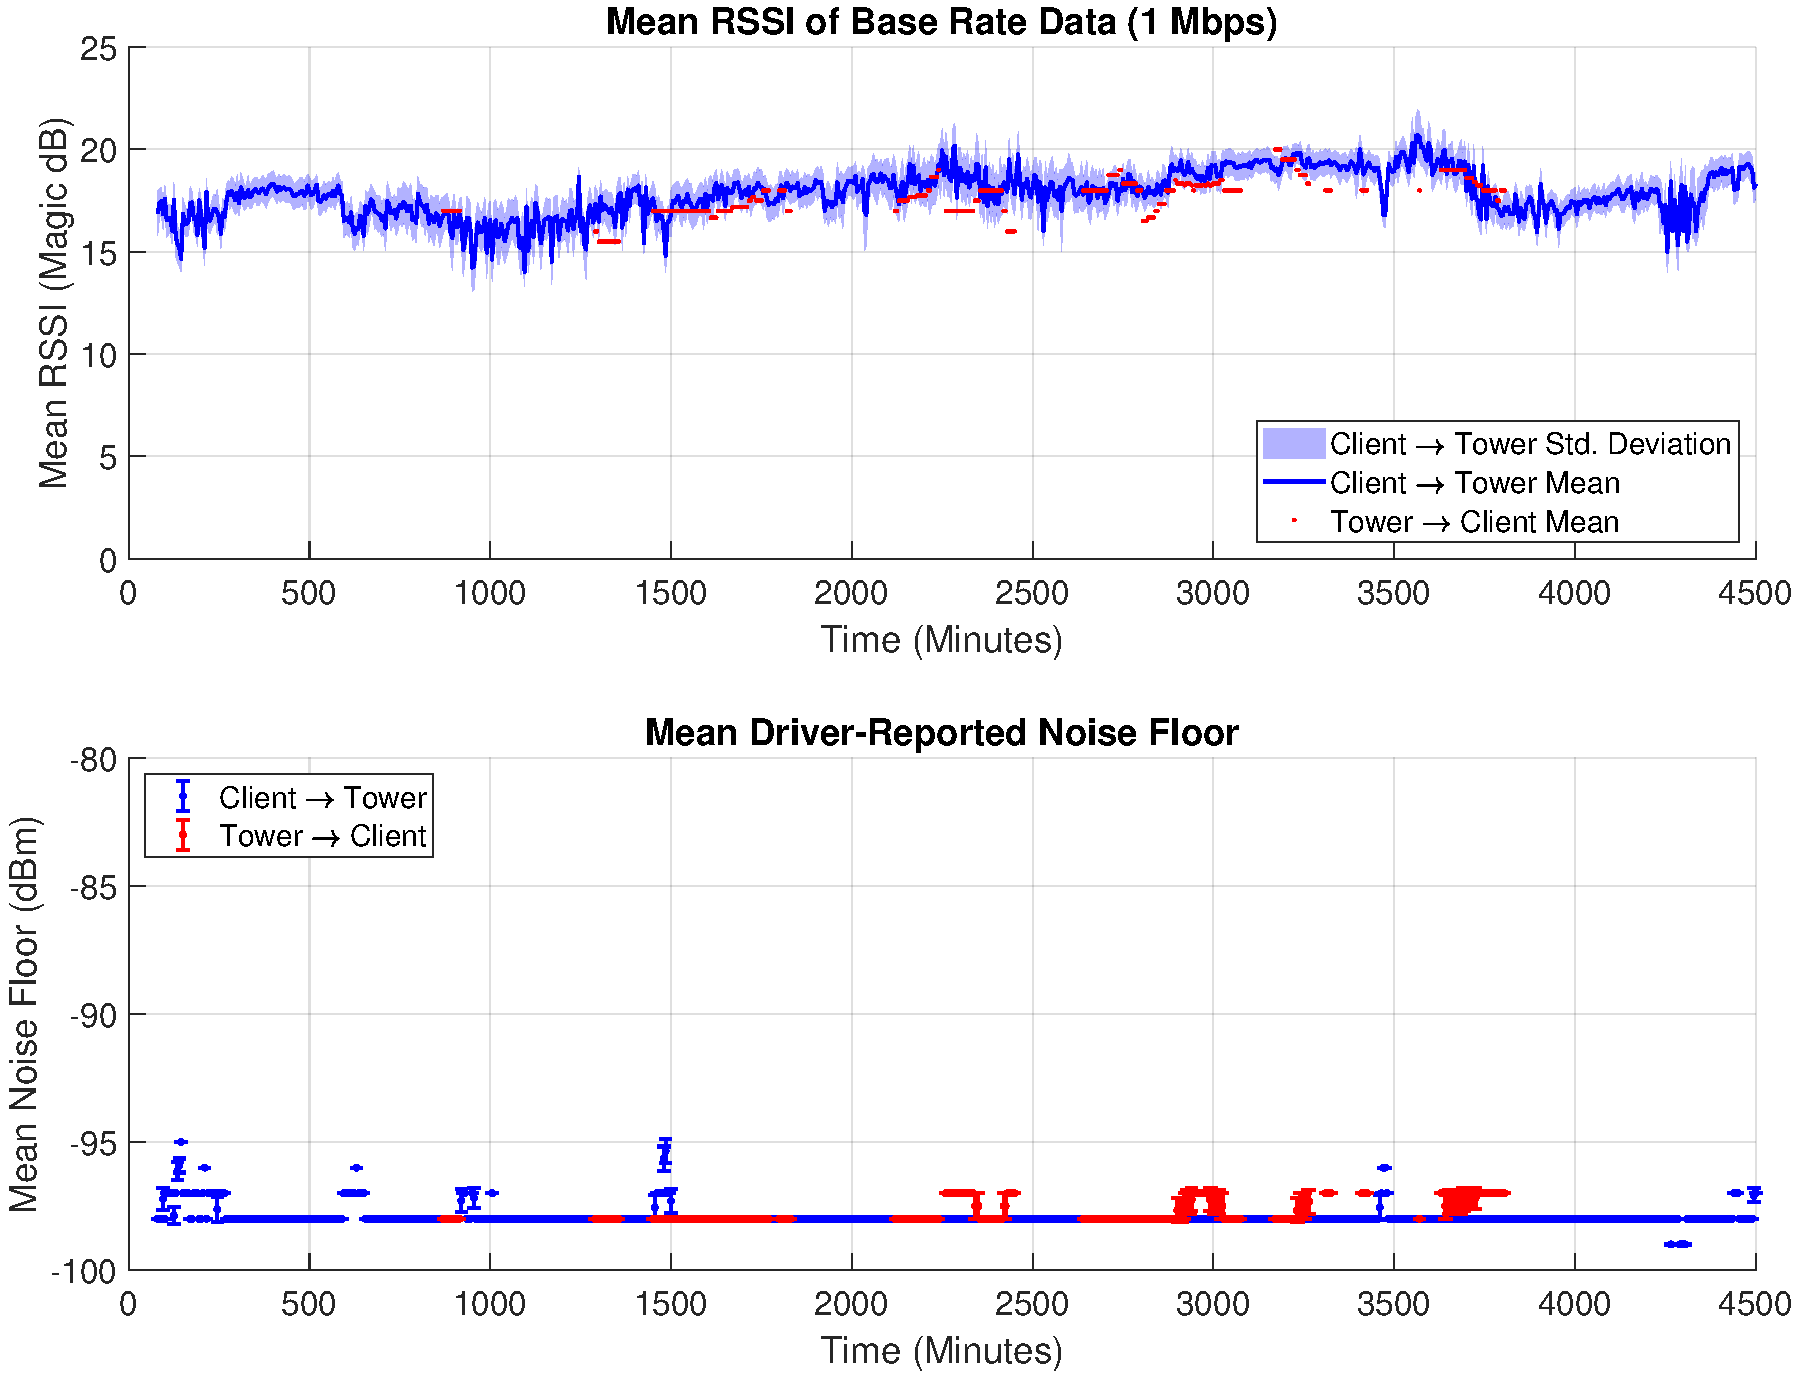
\includegraphics[width=1\linewidth]{figs/wardrive/TFA_long-term-rssi}   
   	\caption{TFA fixed TVWS \ac{RSSI} and noise floor over several days.
	\label{fig_uhf_siso_stability}}
\end{figure}

	The recorded mean uplink \ac{RSSI} value recorded in 5~minute intervals at the ``TFA Tower AP'' from transmissions from the ``Quince St. STA'' nodes shown in Figure~\ref{fig_uhf_rssi_map} is plotted in Figure~\ref{fig_uhf_siso_stability} for the duration of just over 3~days.
	The \ac{STA} was configured to send a base-rate beacon every five seconds; the \ac{RSSI} estimated at the \ac{AP} was recorded and averaged for each 5-minute time interval.
	While we did not have calibration data to relate the measured \ac{RSSI} to an absolute input power to the receiver, we were more interested in relative changes in \ac{RSSI} and were able to confirm that the \ac{RSSI} value reported by our modified ath5k driver was in fact log-linear with respect to power (\textit{i.e.} a 1~dB increase in \ac{RSSI} corresponded to a 1~dB increase in power).
	
	There was only a small window of three days where this experimental topology was able to operate before damage to one of the transceivers impeded operation, however we find that mean signal strength for the \emph{fixed} UHF-band link at 563~MHz varies approximately 5~dB over the course of a few days, where both uplink and downlink \ac{RSSI} measurements appear to agree with each other.
	From one viewpoint, 5~dB can be a large change and requires that care to be taken when provisioning margin in deployment planning; from another viewpoint, the slow and relatively manageable drift in fixed link signal strength can be easily compensated by receiver channel equalizers that are accustomed to compensating for widely varying mobile signal strength.
	The observed signal strength variation at large distances should not be an impediment for large-scale \ac{TVWS} networks.
	
	The recorded data are inconclusive regarding weather effects and diurnal patterns, which would require longer data logs to extract repetitive fluctuations and correlated against known weather patterns.
	Nevertheless, we present our limited data set in order to provide an initial measurement and reference point for future studies on these effects in terrestrial \ac{TVWS} two-way communications.
	

%===============================================
\subsection{Discussion and Conclusion}
\label{sec_siso_conclusion}

	The frequency translation architecture provides a rapid pathway to utilizing \ac{COTS} components to prototype a \ac{TVWS} system; however, it suffers from some severe limitations on performance.

	Firstly, the 802.11b/g standard was designed with relatively lax spectral masks that are inappropriate for \ac{TVWS} systems.
	This leads to large and expensive band-pass filters required for frequency-translation systems that perform the translation in one frequency translation step.
	Since this limits agility, re-designing the frequency translation architecture with a second intermediate frequency for filtering might be necessary for this architecture to be a viable choice.
	
	Second, legacy 802.11 systems scale system capacity by increasing channel bandwidth up to 80+80~MHz, limiting spatial diversity gains to only 4 separate streams maximum according to the 802.11 standard \cite{bejarano2013tutorial}.
	We have shown that the available channel bandwidths in \ac{TVWS} systems operating in the Houston area are fragmented and narrow, which means that we will not be able to practically sustain gigabit network capacity using only 4 spatial streams.
	
	On the positive side, we have shown that there are significant benefits in coverage range of \ac{TVWS} systems compared to other \ac{ISM} bands.
	The ability to deploy fewer towers or installations to cover the same region has a direct impact on the cost and practicality of wireless systems and our evaluation is certainly promising in this regard.
	In order to address the drawback and scaling limits of \ac{SISO} \ac{TVWS} translation architectures, we will now focus on agile \ac{SDR} solutions utilizing \ac{MU-MIMO} techniques.
